\chapter{State of the Art}
\label{chapter:state}

In this chapter we start to describe the technologies and frameworks used for both back-end and front-end implementations, followed by presenting how they interact as a system in the \labelindexref{Implementation}{chapter:implementation} chapter. For serving the web-page we used Django~\ref{sub-sec:django} and for delivering the and the REST API we used a Django compatible extension called Tastypie~\ref{sub-sec:tastypie}, the Django compatible solution. For the display logic and for rendering the front-end components we used Facebook's React.js framework~\ref{sub-sec:react} and also Bootstrap/Flexbox~\ref{sub-sec:bootstrap} for styling.

\section{Back-end Frameworks}
\label{sec:backend}

\subsection{Django}
\label{sub-sec:django}

For our back-end framework we used Django mainly because of it's performance, scalability, stability and the flexibility that it gives to developers. Being a free and open source project, Django benefits of a large community support therefore having an extensive official documentation, a vast collection of tutorials available online and many more extensions available to install trough the built in PIP (Python Package Index) installer.

Django is a web application framework written in Python with a ``batteries-included'' philosophy. The principle behind batteries-included is that the common functionality for building web applications should come with the framework instead of as separate libraries. Therefore, Django can provide developers with all the tools needed to set up a web page. It has a built in relational database for storing information, a templating system for rendering pages and a URL dispatcher for resolving page requests. The framework also comes with more advanced features like XSS (Cross site scripting), CSRF (Cross site request forgery) and SQL Injection protection but also an authentication and admin panel modules.

Django's architecture is described by the developers\footnote{https://docs.djangoproject.com/en/1.8/faq/general/\#django-appears-to-be-a-mvc-framework-but-you-call-the-controller-the-view-and-the-view-the-template-how-come-you-don-t-use-the-standard-names\label{note1}} as a MTV, which stands for ``Model-Template-View,, even if it closely resembles a classic MVC (Model View Controller) pattern which many may be familiar with. A high level view of Django's architecture is shown in \labelindexref{Figure}{img:django-arch}.

\fig[scale=0.3]{src/img/django-arch2.png}{img:django-arch}{Django architecture}

\subsubsection{Model}
\label{sub-sub-sec:model}

The ``Model'' consists of an object-relational mapper that translates data models defined in Python classes to classic relational database tables. Django's default relational database management system is SQLite.

Models are represented by Python classes and contain essential fields and behaviors of the stored data and represent the single source of information about that data. Every class inherits the \texttt{django.db.models.Model} and each model attribute represents a database field \cite{book5}. We present a  very basic example of a \texttt{Book} model class in \labelindexref{Listing}{lst:model-py}.

\lstinputlisting[label={lst:model-py},caption=Book model class,language=Python]{src/code/python/modelexample.py}

We observe that there are two character type fields and one date type field that map to the corresponding columns in \labelindexref{Listing}{lst:model-sql}.

\lstinputlisting[label={lst:model-sql},caption=Book SQL table,language=SQL]{src/code/python/examplesql.sql}

\subsubsection{Template}
\label{sub-sub-sec:template}

The ``Template'' consists of a web templating system that handles the page rendering on the client part. This is also why it is called the ``Template'', even if it basically resembles the MVC ``View'' component. A Django template is composed of static parts of the desired HTML output as well as special syntax that describes how dynamic content will be inserted. An example of rendering a poll question with it's available choices it is presented in \labelindexref{Listing}{lst:template-example}.

\lstinputlisting[label={lst:template-example},caption=Using Django templates,language=html]{src/code/html/template-example.html}

We can see that the Django that trough \texttt{\{\{var\}\}} specific variables are inserted into the HTML that will be generated, like the question text or the choices text. Also, Django provides specific built-in template tags like \texttt{\{\% for in \%\}} for looping over arrays, handling conditional statements, filtering etc.

\subsubsection{View}
\label{sub-sub-sec:view}

The ``View'' is a regular-expression-based URL dispatcher that maps the URL to a view function and calls it. The view function can also check if a cached version of the page is available and skip the following steps. The component was named ``View'' by the developers because the callback function of the dispatcher describes which data is presented to de user. The ``View'' can be seen as an MVC ``Controller'' because the view function performs the requested action, which usually implies reading or writing to the database. An example of a urls.py file that describes the dispatcher, is presented in \labelindexref{Listing}{lst:view-example}.

\lstinputlisting[label={lst:view-example},caption=Urls.py file,language=Python]{src/code/python/view-example.py}

We can see that each URL pattern is matched via the regular expression set as the first parameter of the \texttt{url()} function (eg. \texttt{r'\^{}\$'}) and calls the function callback (the second parameter) with following optional parameters. In the first case the regular-expression will match the empty string with the index function from the views module. The second and third entries will match the paths to the \texttt{posts} api and \texttt{admin} panel view files.



\subsection{Tastypie}
\label{sub-sec:tastypie}

Tastypie\footnote{\url{http://tastypieapi.org/}} is a webservice API framework that comes as an extension application for Django. It provides a convenient, yet powerful and highly customizable abstraction for creating REST-style interfaces. Like Django, Tastypie is an open source, community backed project. Some of it's main features are:

\begin{itemize}
	\item Full GET/POST/PUT/DELETE/PATCH support
	\item Designed to be extended at every turn
	\item Includes a variety of serialization formats (JSON/XML/YAML/bplist)
	\item HATEOAS by default
	\item Well-tested and well-documented
\end{itemize}

Tastypie's basic functionality is taking data represented in the Django models (described by python classes), serializing it and sending the resulted data to the client that consumes the API. During the request/response cycle, Tastypie uses a large portion of the standard Django bahaviour and adds on top of that a ,,hydrate/dehydrate'' cycle. An example for requesting data from a sample endpoint like \texttt{api/v1/author/?format=json} can be summarized as follows:

\begin{itemize}
	\item The Django URL dispatcher checks the requested URL in the \texttt{Resource.urls} and on a match for the list view calls \texttt{Resource.dispatch}
	\item The \texttt{dispatch} method checks if the request is valid by establishing if the used HTTP method is valid. It also checks if the requesting user is authenticated and authorized, and if the resource has a handle  request method. If all checks are passed the \texttt{dispatch} calls \texttt{get\_list}.
	\item The \texttt{get\_list} method fetches the available ModelResource objects, sorts them and applies \texttt{full\_dehydrate} on each one of them.
	\item The \texttt{full\_dehydrate} has the purpose of taking the data from the ModelResource objects and transforming it into a much simpler Tastypie specific data structure, usually a dictionary. Therefore the method applies each object's  \texttt{dehydrate} method to get a simpler data structure for serializing. The process is similar on  POST/PUT/PATCH requests where the \texttt{hydrate} method is applied instead, hence the ,,hydrate/dehydrate'' cycle.
	\item In the end, the \texttt{create\_response} method serializes the data given to it in the requested format (XML, JSON) and returns HttpResponse (200 OK) with the resulted data.
\end{itemize}

\subsubsection{JSON Schema}
\label{sub-sub-sec:json-schema}

Another feature of Django Tastypie is its ability to also provide a JSON Schema of a specific resource. ``JSON Schema defines the media type "application/schema+json", a JSON based format for defining the structure of JSON data. JSON Schema provides a contract for what JSON data is required for a given application and how to interact with it. JSON Schema is intended to define validation, documentation, hyperlink navigation, and interaction control of JSON data.'' \footnote{\url{http://json-schema.org/latest/json-schema-core.html}}

In this project we use the JSON Schema mostly for understanding how the data is structured and act accordingly by generating the right components based on our data. A simple example of a JSON Schema usage is presented in \labelindexref{Listing}{lst:json-schema-demo}. In this example we extracted a simple object from the API used in this project to better describe the purpose of the JSON Schema.Therefore the \texttt{title} object is set with with a \texttt{string} value. The corresponding Schema provides important data about this field like, its \texttt{type},its \texttt{default} value or if the object is editable trough the \texttt{readonly} property.
\\
\lstinputlisting[label={lst:json-schema-demo},caption=Simple JSON Schema,language=Java]{src/code/js/json-schema-demo.js}

\section{Frontend-end Frameworks}
\label{sec:frontend}

\subsection{React}
\label{sub-sec:react}

``React (React.js) is a JavaScript library for creating user interfaces.''\footnote{\label{why-react}\url{http://facebook.github.io/react/docs/why-react.html}} Built at Facebook and Instagram, and later open-sourced to the community (2013), React renders UI components and responds to user events, thus making it resemble the ``View'' component in the MVC architecture style. React aims to solve the problem of ``building large applications with data that changes over time''\textsuperscript{\ref{why-react}}.

The building blocks of React are its \textbf{reusable components}. What makes them so special is the ability to store state and data and to always keep in sync with the UI. As Pete Hunt often says in his talks ``Data changing over time is the root of all evil''\footnote{\url{http://endot.org/notes/2014-01-30-react-rethinking-best-practices/}}, strengthening the idea that the main problem of UI design is knowing in what state it is at a moment in time. By encapsulating state in the components developers were able to reduce coupling and increase cohesion. An example of how a react component is structured is presented in \labelindexref{Listing}{lst:simple-react-component}.

\lstinputlisting[label={lst:simple-react-component},caption=Simple react component,language=JavaScript]{src/code/js/component-demo.js}

In the above example we can see a simple component that describes an HTML input field. Every React component is declared as a React class trough \texttt{React.createClass} function. The most important elements of a React component are:
\begin{itemize}
	\item \texttt{props} - Are usually received from the parent component and should never be modified inside the component's functions as they are the it's single source of truth.
	\item \texttt{state} - Describes the state of the component at a moment in time. The state can \textbf{only} be set at the initial rendering of the component trough \texttt{getInitialState()} function and trough the component \texttt{setState()} function. On any change of the state (resulted by calling the \texttt{setState()} function) the component will call the \texttt{render()} function, thus synchronizing the UI with its current state.
	\item \texttt{render} - The function that actually generates and updates the DOM components. It should never be called by the developer as it is automatically called on specific events such as component initial mount, \texttt{setState()} calls etc. Another feature that can be seen in the example is the return value of the \texttt{render()} function which actually contains some HTML syntax. This is an optional feature of React that js called JSX. The JSX syntax provides developers a more familiar way to describe the DOM elements that they deserve. In \labelindexref{Listing}{lst:simple-react-component} the return value will be compiled by a JSX compiler to the equivalent call:
	\texttt{React.createElement(type:"text", value:this.state.value,\\ onChange:this.handleChange)}.
\end{itemize}

The only data a component will work with are \texttt{props} that are  usually received from its parent component and the component \texttt{state}.

We talked about the React components, the main blocks of the framework but next we will explain how React is structured and how it uses this components to modify the DOM on user actions. In \labelindexref{Figure}{img:react-arch} we present a basic overview of the React architecture. The render cycle can be summarized in four steps:
\fig[scale=0.4]{src/img/react-arch.png}{img:react-arch}{React architecture}

\begin{enumerate}
	\item When the user interacts with the browser it creates an event, for example a button is pressed thus sending a native browser event to the \texttt{ReactEvent} system.
	\item  Browser events may not be standardized between certain browsers so React takes this event, normalizes it to the W3C standards and creates a \texttt{Synthetic event} that is dispatched to the components that have a callback set on that event in the \texttt{User code}.
	\item Next, the user code (that runs inside a react component) may change its state and call \texttt{setState()} thus triggering a re-render. At this step react creates a \texttt{Descriptor} with the element that has changed in the Virtual DOM (which we will explain next in more detail) and sends it to the \texttt{ReactDiff} algorithm.
	\item Finally the \texttt{ReactDiff} algorithm computes the minimum number of DOM mutations and sends the operations back to the browser.
\end{enumerate}


\subsubsection{Virtual DOM}
\label{sub-sub-sec:virtual-dom}

As mentioned before, React holds a JavaScript in-memory representation of the web-page's DOM, called a \textbf{Virtual DOM}. As shown in \labelindexref{Figure}{img:react-dom}, React components will first mutate the Virtual DOM that will later be used for diffing. With this new Virtual DOM, the React diffing algorithm must compute the minimum number of operations needed to transform a tree into another and apply the mutation operations to the real DOM.

\fig[scale=0.4]{src/img/react-dom-update.png}{img:react-dom}{React DOM update}

This diffing operation may seem time consuming and inefficient, considering that even some of the best algorithms for tree editing have a complexity of $O(n^3)$\cite{trees} (where $n$ are the number of tree nodes). Therefore React implements a $O(n)$ algorithm using heuristics based on two assumptions\footnote{\url{https://facebook.github.io/react/docs/reconciliation.html}}:

\begin{itemize}
	\item We can assume that two components of the same class will generate similar trees and if they are of different classes they will generate different trees.
	\item Developers can provide unique keys for the components that will not change between different renders so operations on lists of items can be done faster.
\end{itemize}




\subsection{Bootstrap/Flexbox}
\label{sub-sec:bootstrap}

For styling our HTML components we used the Bootstrap framework to achieve an experience similar to a real product. For laying out and aligning the panels that are auto-generated by exploring the Tastypie resource, we used the Flexbox module. 

\subsubsection{Bootstrap}
\label{sub-sub-sec:bootstrap}

Bootstrap is a powerful front-end framework created at Twitter by Mark Otto and Jacob Thornton\footnote{\url{https://github.com/twbs/bootstrap}}, that features a rich collection of tools for faster development and quality work. The most appreciated features are the custom HTML and CSS components, plenty javascript plugins and a popular responsive page layout system. The project is also an open-source community backed project and it's main goal is to ease web development by giving the developers the ability to have consistent styling with minimum effort.

With Bootstrap we can simply structure the DOM with components like Panels by setting custom classes on the elements. An example is shown in \labelindexref{Listing}{lst:bootstrap} and the resulted component in \labelindexref{Figure}{img:bootstrap-panel}.

\lstinputlisting[label={lst:bootstrap},caption=Panel with title ,language=html]{src/code/html/panel.html}

\fig[scale=0.5]{src/img/bootstrap-panel.png}{img:bootstrap-panel}{Panel with title}


\subsubsection{Flexbox}
\label{sub-sub-sec:flexbox}

The Flexbox Layout (Flexible Box) module was built in the CSS3 standard, with the main goal of trying to properly alter width/height of items inside of a container, even if their sizes were unknown, hence the ``flexible box'' naming.

In the flex layout model, the children of a flex container can be laid out in any direction, and can “flex” their sizes, either growing to fill unused space or shrinking to avoid overflowing the parent\cite{flexbox}. An overview of the flex container is presented in \labelindexref{Figure}{img:flexbox}.

We can see the main flex container being populated by flex items. In the flex layout the items will be laid out following either the \texttt{main axis} (from \texttt{main-start} to \texttt{main-end}) or the \texttt{cross axis} (from \texttt{cross-start} to \texttt{cross-end}).

%\fig[scale=0.4]{src/img/flexbox-remake.png}{img:flexbox}{Flex container}

\begin{figure}[H]
	\centering
	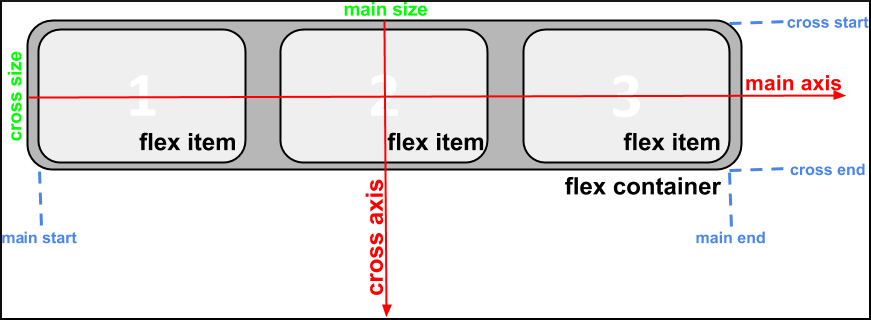
\includegraphics[scale=0.4]{src/img/flexbox-remake.png}
	\caption{Flex container\label{img:flexbox}}
\end{figure}

The container has a collection of properties for laying out the items like: \texttt{flex-direction, flex-wrap, flex-flow, align-content, align-items, justify-content} which can be used for item layout and alignment. An example using two of these is presented in \labelindexref{Listing}{lst:flex-flow} and \labelindexref{Figure}{img:flexbox2}.

\lstinputlisting[label={lst:flex-flow},caption=Flexbox flex-flow usage ,language=html]{src/code/html/flex-flow.html}

\fig[scale=0.25]{src/img/flexbox-flex-flow.png}{img:flexbox2}{Flex-flow usage result}

The \texttt{flex-flow} property is a shorthand for \texttt{flex-direction} and \texttt{flex-wrap} properties. It first establishes the main axis and direction of the layout (\texttt{row-reverse}), the opposite of inline direction, and sets the items to wrap if they don't fit on the same row in the upwards direction (\texttt{upwards}).